\section{Tests}

\begin{frame}{Tests}

  Chose to evaluate specific features of our solution

  \vfill{}

  Studied some network metrics and non-functional requirements

  \vfill{}

  Openstack virtual machines specification
  \begin{itemize}
    \item Receiver with 32GB of RAM, 8vCPU and solid state storage
    \item 4 machines for Kubernetes cluster with 16GB of RAM, 6vCPU and solid state storage
    \item Sender with 4GB of RAM, 2vCPU and solid state storage
  \end{itemize}

\end{frame}

\begin{frame}{Tests - RTT}

  \vspace{-1cm}

  \begin{figure}[H]
    \centering
    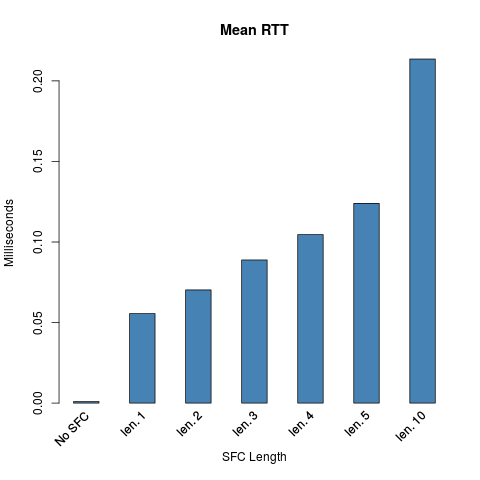
\includegraphics[scale=0.3]{meanrtt}
  \end{figure}

  \begin{itemize}
  \item RTT is higher using the SFC platform
  \item Time is required to elaborate and exchange packets
  \item Linear increase even due to the usage of the safe function
  \end{itemize}

\end{frame}

\begin{frame}{Tests - Time to recover from a fault}

  \vspace{-1cm}

  \begin{figure}[H]
    \centering
    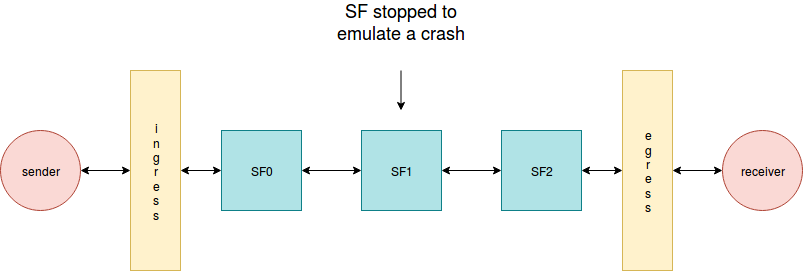
\includegraphics[scale=0.3]{testfaultconf}
  \end{figure}

  \begin{itemize}
  \item after 5s that the sender starts to send packet the VNF is stopped
  \item about 13s required to restore a faulty container
  \item both using TCP and UDP
  \end{itemize}

\end{frame}